\documentclass[18pt, aspectratio=169, handout]{beamer}
\usepackage[ngerman]{babel}
\usepackage[final]{microtype}
\usepackage[T1]{fontenc}
\linespread{1.05}

\usepackage{xcolor}
\usepackage{lmodern}
\usepackage{amssymb}
\usepackage{amsmath}
\usepackage{mathtools}
\usepackage{unicode-math}
\defaultfontfeatures{Ligatures=TeX,Scale=MatchLowercase}
\let\emptyset\varnothing

\usepackage{url}
\usepackage{graphicx}
\usepackage{svg}
%\usepackage{tabularx}

\setlength{\parindent}{0pt}
\setlength{\parskip}{6pt plus 2pt minus 1pt}

\usepackage{hyperref}
\hypersetup{pdfborder={0 0 0},breaklinks=true}

%\usepackage{enumitem}
%\setlist[itemize]{noitemsep}

\usepackage{fontspec}
\newfontfamily\univers{Univers LT 45 Light}[
  SmallCapsFont=CMU Sans Serif,
  SmallCapsFeatures={Letters=SmallCaps}
]

\usepackage{cite}
\renewcommand{\citeleft}{}
\renewcommand{\citeright}{}

\setbeamertemplate{navigation symbols}{}
\setbeamertemplate{footline}[frame number]

\setbeamertemplate{itemize item}{\_}
\setbeamertemplate{itemize subitem}{\_}
\setbeamertemplate{itemize subsubitem}{\_}

\setbeamercolor{titlelike}{fg=black}
\setbeamercolor{framesubtitle}{fg=gray}
\setbeamerfont{frametitle}{size=\small,series=\bfseries}
\setbeamerfont{framesubtitle}{size=\normalfont\small}

\setbeamercolor{structure}{fg=black}
%\setbeamercolor{bibliography item}{fg=black}
\setbeamercolor{bibliography entry author}{fg=black}
\setbeamercolor{bibliography entry title}{fg=black} 
\setbeamercolor{bibliography entry location}{fg=black} 
\setbeamercolor{bibliography entry note}{fg=black}  

\defbeamertemplate*{title page}{customized}[1][]{%
  \bigskip
  {\Huge\bfseries\inserttitle\par}
  {\Large\insertsubtitle\par}
  \vspace{2\bigskipamount}
  {\normalsize\insertauthor\par}
  \begin{figure}[b]
  	\hspace{6cm}
  	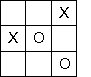
\includegraphics{tic_single_titleframe.pdf}
  \end{figure}
  \bigskip
  \small \insertinstitute\\
  \insertdate\par
}

\newcommand\e[1]{\begin{em}#1\end{em}}
\newcommand\q[1]{\glqq #1\grqq}
\newcommand\sq[1]{\glq #1\grq}
\newcommand\qq[1]{\glqq\e{#1}\grqq}
\newcommand\fnm[1]{\footnotemark[#1]\addtocounter{footnote}{1}}
\newcommand\tu[1]{\quad{\tiny\url{#1}}}
\newcommand\tuu[1]{{\tiny\url{#1}}}
\newcommand\citeh[1]{\textsuperscript{\cite{#1}}}

\newcommand\g[3]{%
  \begin{figure}[!ht]
  \centering
  \includegraphics[width=#2\textwidth]{#1}
  {\small#3}
  \end{figure}}
\newcommand\gsvg[3]{%
  \begin{figure}[!ht]
  \centering
  \includesvg[width=#2\textheight]{#1}
  {\small#3}
  \end{figure}}
\newcommand\gw[2]{%
  \begin{figure}[!ht]
  \centering
  \includegraphics[width=0.8\textwidth]{#1}
  {\small#2}
  \end{figure}}
\newcommand\gh[2]{%
  \begin{figure}[!ht]
  \centering
  \includegraphics[height=0.8\textheight]{#1}
  {\small#2}
  \end{figure}}

\newcommand\todo[1]{\colorbox{yellow}{\tiny\textsc{ToDo: }#1}\\}


\subtitle{Vortrag zum Thema Spielbäume}
\author{Joschka Heinrich}
\institute{Proseminar Theoretische Informatik\\Fakultät Informatik, TU Dresden}
\date{15.02.2018}

\begin{document}
\univers
\begin{frame}[plain]
	\title{Tic-Tac-Toe like a Pro}
  \maketitle
\end{frame}

\begin{frame}[plain]
	\title{Tic-Tac-Toe like a Bro}
  \maketitle
\end{frame}

\title{Tic-Tac-Toe like a Pro}


%%%%%%%%%%%%%%%%%%%%%%%%%%%%%%%%%%%%%%%%%%%%%%%%%%%%%%%%%%%%%%%%%%%%%%%%%%%%

\begin{frame}{Unsere Fragestellung}{Motivation}
  \begin{center}
  	\Large\textbf{Wie wähle ich in einem Spiel den günstigsten Zug?}
	\end{center}
\end{frame}

\begin{frame}{Agenda}{\inserttitle}
  \gw{a/agenda_diagram.pdf}{}
\end{frame}

\begin{frame}{Donald Michies \q{Menace}}{Motivation}
  \only<1>{\gh{img/michie.png}{\_ Donald Michies, 2003\citeh{img_michie}}}
  \pause
  \gw{img/menace.png}{\_ Menace, 1963\citeh{img_menace}}
\end{frame}

%\begin{frame}{Kreuze und Kreise}{Motivation}
%	\only<1>{\gh{img/TicX.pdf}{\_ Beste Züge aus Sicht von X\citeh{img_ticx}}}
%	\pause
%	\gh{img/TicO.pdf}{\_ Beste Züge aus Sicht von O\citeh{img_tico}}
%\end{frame}

\begin{frame}{Lernziele dieses Vortrages}{Motivation}
  \begin{itemize}
		\item
		  formale Betrachtung von \textbf{Spielen} verstehen
		  \pause
		\item
		  \textbf{Minmax-Algorithmus} nachvollziehen können
		  \pause
  	\item
		  gute und schlechte \textbf{Heuristiken} unterscheiden und anwenden können
		  \pause
		\item
		  Vorteile der \textbf{Alpha-Beta-Kürzung} verstehen
	\end{itemize}
\end{frame}


%%%%%%%%%%%%%%%%%%%%%%%%%%%%%%%%%%%%%%%%%%%%%%%%%%%%%%%%%%%%%%%%%%%%%%%%%%%%

\begin{frame}{Terminologie}{Spiel, Konfiguration, Spielbaum}
  \gw{a/agenda_diagram_Term.pdf}{}
\end{frame}

\begin{frame}{Zufall und Information}{Terminologie}
	\g{img/spiel.pdf}{0.65}{}
\end{frame}

\begin{frame}{Spiel, Spielzug, Konfiguration}{Terminologie}
	\begin{itemize}
		\item zwei Spieler: \textbf{Max} und \textbf{Min}
		\pause
		\item Nullsummenspiel
		\pause
		\item $K$ \quad Menge aller \textbf{zulässigen Konfigurationen}
		\pause
		\item Spiel $S \coloneqq (R,k_0,F)$
		\begin{itemize}
			\pause
			\item $R$ \quad Menge \textbf{legaler Spielzüge}
			\pause
			\item $k_0 \in K$ \quad \textbf{Anfangskonfiguration}
			\pause
			\item $F \subset K$ \quad Menge der \textbf{Endkonfigurationen}
		\end{itemize}
	\end{itemize}	
\end{frame}

\begin{frame}{Spielzüge als Funktion, Folgekonfiguration}{Terminologie}
	\begin{itemize}
		\item $R:K^2,~r$ legal
		\pause
		\begin{itemize}
			\item wenn $v = r(u)$, dann heißt $v$ \textbf{Kindkonfiguration} von $u$ (bezüglich $r$)
			\item analog: $u$ \textbf{Elternkonfiguration} von $v$ (bezüglich $r$)
		\end{itemize}
		\pause
		\item $R_k \coloneqq \{r \in R \mid r$ anwendbar auf $k\}$
		\pause
		\item \textbf{Menge der Kindkonfigurationen} $N(k) \coloneqq \{r(k) \mid r \in R_k\} \subseteq K$
		\pause
		\begin{itemize}
			\item $N(k_f) = \emptyset,~k_f \in F$
		\end{itemize}
		\pause
		\item $K$ induktiv über Kindkonfiguration definierbar:
		\pause
		\begin{itemize}
			\item[(1)] $k_0 \in K$
			\item[(2)] $\forall k \in K: N(k) \subset K$
		\end{itemize}
	\end{itemize}
\end{frame}

\begin{frame}{mögliche, legale und anwendbare Spielzüge}{Terminologie}
	\g{img/spielzuege.pdf}{1}{}
\end{frame}

\begin{frame}{Spielbaum}{Terminologie}
	\begin{itemize}
		\item \textbf{Spielbaum} ist gerichteter Graph $G_S \coloneqq (V,E)$ 
		\pause
		\begin{itemize}
			\item Knoten $V = K$
			\pause
			\item Kanten $E = \bigcup\limits_{u \in K}\{(u,v) \mid v \in N(u)\}$
		\end{itemize}

		\pause
		\item $G_S$ ist Baum mit Wurzel $k_0$, Blättern $F$
		\pause
		\item Spielverlauf mit $l$ Zügen ist Pfad $p$ subsequenter Kindkonfigurationen
		\begin{itemize}
			\item $p = (k_0,k_1,\dots,k_l)$
		\end{itemize}
		\item zu große Komplexität
	\end{itemize}
\end{frame}

\begin{frame}{Tic-Tac-Toe-Spielbaum der Tiefe 2}{Terminologie}
	\begin{figure}[!ht]
  \centering
  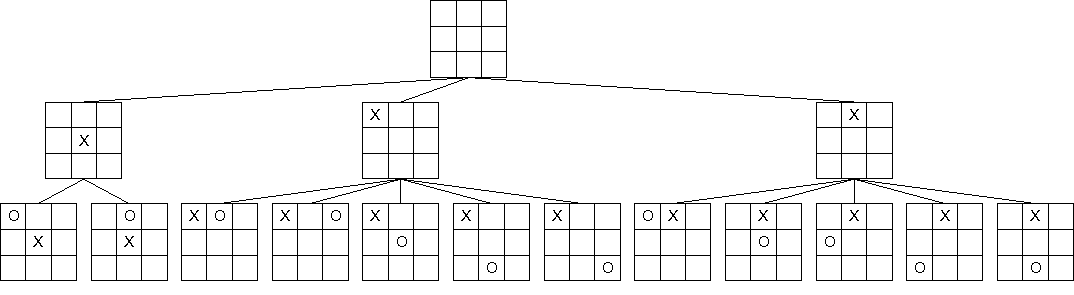
\includegraphics[width=\textwidth]{tic.pdf}
  \end{figure}
\end{frame}


%%%%%%%%%%%%%%%%%%%%%%%%%%%%%%%%%%%%%%%%%%%%%%%%%%%%%%%%%%%%%%%%%%%%%%%%%%%%

\begin{frame}{Minmax}{Geschichte, Algorithmus, Komplexität}
  \gw{a/agenda_diagram_MinMax.pdf}{}
\end{frame}

\begin{frame}{Geschichte des Minmax-Algorithmus}{Minmax}
	\begin{itemize}
		\item populär als Suchalgorithmus für Spielstrategie in Schachprogrammen
		\item 1912 erstmals von Ernst Zermelo erwähnt
		\item 1940er: Bedeutung von Minmax betont (Shannon, Turing)
	\end{itemize}

  \begin{columns}
	  \column[t]{.5\textwidth}
	  \g{img/shannon.jpg}{0.35}{\\\_ Claude Shannon, 1963\citeh{img_shannon}}
	  
	  \column[t]{.5\textwidth}
	  \g{img/turing.jpg}{0.35}{\\\_ Alan Turing, 1928\citeh{img_turing}}

  \end{columns}
\end{frame}

\begin{frame}{Voraussetzungen für den Algorithmus}{Minmax}
	\begin{itemize}
	\item
	  zwei Typen von Knoten
	  \pause
	  \begin{itemize}
	  	\item Max ist am Zug: \textbf{Max-Knoten} \quad $\bigtriangleup$
	  	\item Min ist am Zug: \textbf{Min-Knoten} \quad $\bigtriangledown$
		  \item Min/Max alternierend in jedem Halbzug
  	\end{itemize}
  	\pause
  	\item jedem Knoten im Baum wird ein Minmax-Wert zugeordnet
  	\begin{itemize}
  		\item entspricht Max' \textbf{Nutzen dieser Konfiguration}
		\end{itemize}
		\pause
		\item Minmax-Wert des Knotens $k$ ergibt sich aus Minmax-Werten der Kinder $N(k)$\\ $\rightarrow$ \textbf{Tiefensuche} (\textit{depth first})
		\pause
		\item Gewinnfunktion $g: F \to \mathbb{N}$, die Endkonfigurationen bewertet\\(aus Sicht von Max)
	\end{itemize}
\end{frame}

\begin{frame}{Der Minmax-Algorithmus}{Minmax}
$Minmax(u) = \Bigg\{$
	  \begin{tabular}{ll}
		  $g(u)$ & wenn $u \in F$\\
		  $max_{v \in N(u)} Minmax(v)$ & wenn Max in $u$ am Zug\\
		  $min_{v \in N(u)} Minmax(v)$ & wenn Min in $u$ am Zug
	  \end{tabular}

	  \vspace{2\baselineskip}
	  \pause

	\begin{itemize}
    \item
      Max-Knoten: Max wählt besten Zug \\
      $\rightarrow$ \textbf{höchsten} Wert annehmen
    \item
      Min-Knoten: bester Zug für Min ist schlechtester für Max \\
      $\rightarrow$ \textbf{kleinsten} Wert für Max annehmen
  \end{itemize}
\end{frame}

\begin{frame}{Minmax bei Tic-Tac-Toe}{Minmax}
	\only<1>{\gh{img/tic_minmax.pdf}{}}
	\only<2->{\gh{img/tic_minmax_2.pdf}{}}
	\pause
\end{frame}

\begin{frame}{Abstrakter Minmax-Bäume}{Minmax}
	\gw{minmax.pdf}{}
\end{frame}

\begin{frame}{Komplexität}{Minmax}
	\begin{itemize}
		\item
		  $m$ \quad \textbf{maximale Tiefe} des Spielbaumes
		\item
		  $b$ \quad \textbf{Verzweigungsgrad}
		  \pause
		\item
		  Zeitkomplexität: $\mathcal{O}(b^m)$
		\item
		  Speicherkomplexität: $\mathcal{O}(bm)$, bzw. $\mathcal{O}(m)$
	\end{itemize}
\end{frame}


%%%%%%%%%%%%%%%%%%%%%%%%%%%%%%%%%%%%%%%%%%%%%%%%%%%%%%%%%%%%%%%%%%%%%%%%%%%%

\begin{frame}{Unvollständige Echtzeitentscheidungen}{Heuristik, Expansionskriterium}
  \gw{a/agenda_diagram_Echt.pdf}{}
\end{frame}

\begin{frame}{Verbesserung Minmax}{Unvollständige Echtzeitentscheidung}
	\begin{itemize}
	\item
	  neu: \textbf{Kriterium}, wann Knoten expandiert werden soll
	  \pause
	\item
	  \textbf{Heuristik}, um nicht-Endkonfiguration zu bewerten
	  \pause
	\item
	  Stärke des Agenten hängt ab von:
	  \begin{itemize}
	  \item[(a)] Bewertung des Nutzens einer Knotenexpansion
	  \item[(b)] Genauigkeit der Heuristik
		\end{itemize}
	\end{itemize}
\end{frame}

\begin{frame}{Heuristiken}{Unvollständige Echtzeitentscheidung}

\begin{itemize}
\item
  Heuristik schätzt Nutzen für Spieler in bestimmter Konfiguration
  \begin{itemize}
  	\item vergleichbar mit $A^*$-Suche
  \end{itemize}
  \pause
  \item
  aus Merkmalen der Konfiguration zusammengesetzt
	\item
	\pause
  Anforderungen:
  \begin{itemize}
  \item
    muss gleiche Ordnung wie Gewinnfunktion erzeugen
    \pause
  \item
    muss effizient sein
    \pause
  \item
    muss für nicht-Endkonfigurationen Wert nahe der \textit{tatsächlichen} Chance liefern
  \end{itemize}
\end{itemize}
\end{frame}

\begin{frame}{Eine Heuristik für TicTacToe}{Unvollständige Echtzeitentscheidung}
	\begin{itemize}
  	\item $f(k) = A_X(k) - A_O(k)$
  		\begin{itemize}
  			\item $A_{X/O}(k)$ \quad \q{Wie viele Möglichkeiten zur Verfollständigung von Linien gibt es?}
  		\end{itemize}
  \end{itemize}
\end{frame}

\begin{frame}{Noch einmal Tic-Tac-Toe}{Terminologie}
	\only<1>{%
	\begin{figure}[!ht]
  \centering
  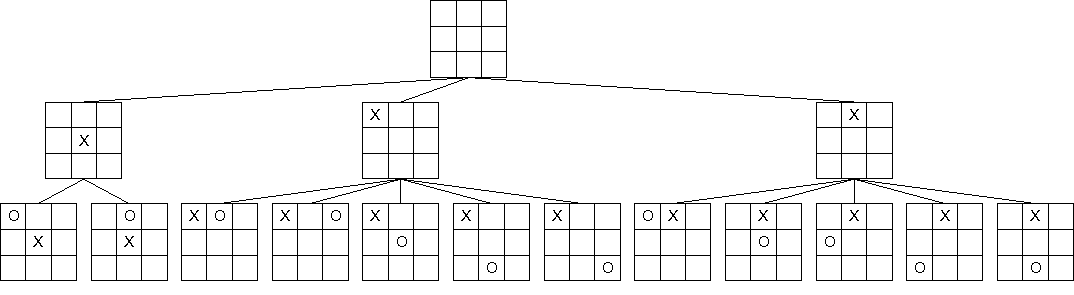
\includegraphics[width=\textwidth]{tic.pdf}
  \end{figure}}
  \only<2>{\g{minmax_heuristik.pdf}{1}{}}
  \only<3>{\g{minmax_heuristik_2.pdf}{1}{}}
  \pause
  \pause
\end{frame}

\begin{frame}{Expansionskriterium}{Unvollständige Echtzeitentscheidung}
\begin{itemize}
\item
  trivial: immer terminieren, wenn Endkonfiguration erreicht ist
\item
  Metaschluss: Wann lohnt es sich, eine Berechnung anzustellen?
\item
  Beispiele
  \begin{itemize}
  	\item feste Tiefe $l$
    \item \textbf{Ruhesuche:} Bewertung ändert sich nicht mehr stark
  \end{itemize}
\end{itemize}
\end{frame}


%%%%%%%%%%%%%%%%%%%%%%%%%%%%%%%%%%%%%%%%%%%%%%%%%%%%%%%%%%%%%%%%%%%%%%%%%%%%

\begin{frame}{$\alpha,\beta$}{Geschichte, Algorithmus, Komplexität}
  \gw{a/agenda_diagram_AlphaBeta.pdf}{}
\end{frame}

\begin{frame}{Geschichte der Alpha-Beta-Kürzung (auch $\alpha$-$\beta$-Pruning, -Suche)}{$\alpha,\beta$}
  \begin{columns}
	  \column[t]{.5\textwidth}
		\begin{itemize}
			\item Optimierung von Minmax
			%\item von verschiedenen Personen entwickelt{\tiny\\(Samuel, Richards, Hart, Levine, Edwards, Brudno, \dots)}
			\item 1956 in Dartmouth vorgestellt (McCarthy)\\~
		\end{itemize}
	  
	  \g{img/mccarthy.png}{0.4}{\\\_ John McCarthy, 1967\citeh{img_mccarthy}}
	  
	  \column[t]{.5\textwidth}
		\begin{itemize}
			\item 1961 erstmals in Schachprogramm eingesetzt
			\item 1975 verfeinert (Knuth, Moore)
		\end{itemize}
	
	  \g{img/knuth.jpg}{0.4}{\\\_ Donald E. Knuth, 2005\citeh{img_knuth}}
  \end{columns}
\end{frame}



\begin{frame}{Erweiterung von Minmax}{$\alpha,\beta$}
  \begin{itemize}
	  \item
	    einen Alpha- und einen Beta-Wert für jeden Knoten
	    \pause
	  \item
	    \textbf{untere Schranke} $\alpha$ für Maxknoten
  	\begin{itemize}
  		\item bisher größte Bewertung im Pfad zu $k$
  	\end{itemize}
  	\pause
	  \item
	    \textbf{obere Schranke} $\beta$ für Minknoten
	    \begin{itemize}
  		\item bisher kleinste Bewertung im Pfad zu $k$
  	\end{itemize}
		\pause
  	\item
	  $\alpha$ und $\beta$ werden nach jeder untersuchten Konfiguration
	  aktualisiert

	  \begin{itemize}
	  \item
	    initial $\alpha = -\infty$, $\beta = +\infty$
	  \item
	    $\alpha$ wird an einem Max-Knoten maximiert
	  \item
	    $\beta$ wird an einem Min-Knoten minimiert
	  \end{itemize}
  \end{itemize}
\end{frame}


\begin{frame}{Kürzung}{$\alpha,\beta$}
\begin{itemize}

\item
  \textbf{Kürzung} der Kindknoten, \\d.h. die Rekursion \textit{vor} Erreichen der Endkonfiguration terminiert
\pause
  \item
    an Max-Knoten \textbf{$\alpha$-Cut}
    \begin{itemize}
    	\item es wird der größte Wert unter den Kindern gesucht
      \item sobald $\beta$ eines Kindes $\leq \alpha$
    \end{itemize}
    \pause
  \item
    an Min-Knoten \textbf{$\beta$-Cut}
    \begin{itemize}
    	\item es wird der kleinste Wert unter den Kindern gesucht
      \item sobald $\alpha$ eines Kindes $\geq \beta$
    \end{itemize}
\end{itemize}

\end{frame}


\begin{frame}{Ein $\alpha,\beta$ Beispiel}{$\alpha,\beta$}
\only<1>{\g{minmax_alphabeta_1.pdf}{.8}{}}
\only<2>{\g{minmax_alphabeta_2.pdf}{.8}{}}
\only<3>{\g{minmax_alphabeta_3.pdf}{.8}{}}
\only<4>{\g{minmax_alphabeta_4.pdf}{.8}{}}
\only<5>{\g{minmax_alphabeta_5.pdf}{.8}{}}
\only<6>{\g{minmax_alphabeta_6.pdf}{.8}{}}
\pause
\pause
\pause
\pause
\pause
\end{frame}

\begin{frame}{Komplexität}{$\alpha,\beta$}
\begin{itemize}
\item
  Minmax: $\mathcal{O}(b^m)$
\item
  Alpha-Beta-Kürzung: $\mathcal{O}(b^{\frac{m}{2}})$
  \begin{itemize}
  \item bei optimaler Sortierung (\textbf{Zugreihenfolge})
  \item theoretisches Limit, wenn immer sofort gekürzt werden kann
  \item bei zufälliger Sortierung der Knoten: $\mathcal{O}(b^{\frac{3}{4}m})$
  \end{itemize}
\end{itemize}
\end{frame}


%%%%%%%%%%%%%%%%%%%%%%%%%%%%%%%%%%%%%%%%%%%%%%%%%%%%%%%%%%%%%%%%%%%%%%%%%%%%

\begin{frame}{Ausblick}{Zugreihenfolge}
  \g{a/agenda_diagram_Ausblick.pdf}{0.5}{}
\end{frame}

\begin{frame}{Zugreihenfolge}{Ausblick}
  \begin{itemize}
  \item
    vorsortieren und Killerzüge finden ("Killerzugheuristik")
  \item
    dynamisch: zuerst Züge probieren, die vorher gut waren
    \begin{itemize}
    \item
      Situationen können wieder auftreten $\rightarrow$ Hashtabelle anlegen
    \end{itemize}
  \end{itemize}
\end{frame}


\begin{frame}{Verbesserung mit iterativer Tiefensuche}{Ausblick}
  \begin{itemize}
  	\item Suchtiefe mit jedem Durchlauf erhöhen
  	\pause
  \item
    hilft bei Wahl einer günstigen Zugreihenfolge
  \item
    nutzt begrenzte Zeit best möglich aus
  \end{itemize}
\end{frame}

\begin{frame}{Rückblick}{zur Motivation}
  \begin{itemize}
		\item
		  formale Betrachtung von \textbf{Spielen} verstehen
		\item
		  \textbf{Minmax-Algorithmus} nachvollziehen können
  	\item
		  gute und schlechte \textbf{Heuristiken} unterscheiden und anwenden können
		\item
		  Vorteile der \textbf{Alpha-Beta-Kürzung} verstehen
	\end{itemize}
\end{frame}



\begin{frame}{}{}
  \begin{center}
  joschka.heinrich@tu-dresden.de\\

  \vspace{\baselineskip}
  B40E 67C7 FF62 C860 7854 A778 6FB9 666F 1147 A401\\
  \vspace{\baselineskip}

  \g{img/github.png}{0.2}{\\\url{https://github.com/foobar0112/tic}}
  \end{center}
\end{frame}


%%%%%%%%%%%%%%%%%%%%%%%%%%%%%%%%%%%%%%%%%%%%%%%%%%%%%%%%%%%%%%%%%%%%%%%%%%%%


\begin{frame}{Sachquellen}{Anhang}
  \begin{itemize}
    \item Klüppelholz: \q{Entwurfs- und Analysemethoden für Algorithmen -- Skript zur Vorlesung SS 2016}
    \item Russel, Norvig: \q{Künstliche Intelligenz -- Ein moderner Ansatz}, 3., aktualisierte Auflage, 2012
    \item \url{http://chalkdustmagazine.com/features/menace-machine-educable-noughts-crosses-engine}
    \item \url{https://de.wikipedia.org/wiki/Tic-Tac-Toe}
		\item \url{https://en.wikipedia.org/wiki/Tic-tac-toe}
		\item \url{https://de.wikipedia.org/wiki/Minimax-Algorithmus}
		\item \url{https://en.wikipedia.org/wiki/Minimax}
		\item \url{https://de.wikipedia.org/wiki/Alpha-Beta-Suche}
		\item \url{https://en.wikipedia.org/wiki/Alpha-beta_pruning}
  \end{itemize}
\end{frame}

\begin{frame}{Bildquellen}{Anhang}
  \setbeamertemplate{bibliography item}[text]
  \begin{thebibliography}{99}
		\bibitem{img_michie} Donald Michies \tu{http://www.aiai.ed.ac.uk/~dm/donald-michie-2003.jpg}
		\bibitem{img_menace} Menace \tu{http://images.slideplayer.nl/9/2257151/slides/slide_6.jpg}
		\bibitem{img_shannon} Claude Shannon \tu{https://upload.wikimedia.org/wikipedia/commons/9/99/ClaudeShannon_MFO3807.jpg}
		\bibitem{img_turing} Alan Turing \tu{https://upload.wikimedia.org/wikipedia/commons/a/a1/Alan_Turing_Aged_16.jpg}
		\bibitem{img_mccarthy} John McCarthy \tu{http://images.computerhistory.org/fellows/2-4a.stanford_university.mccarthy-john.c1967.l062302006.stanford_university.src.jpg}
		\bibitem{img_knuth} Donald E. Knuth \tu{https://upload.wikimedia.org/wikipedia/commons/4/4f/KnuthAtOpenContentAlliance.jpg}
	\end{thebibliography}
\end{frame}


\begin{frame}{Suchbaum $\nequiv$ Spielbaum}{Anhang}
	\begin{itemize}
		\item \textbf{Suchbaum} ist gerichteter Graph $(V,E,l,w)$, Baum
		\begin{itemize}
			\item Tiefe $l \in \mathbb{N}_{> 0}$
			\item Knoten entsprechen Pfaden der maximalen Länge $l$, ausgehend von $w$ im \textit{Spiel}baum
			\item Kanten entsprechen anwendbarem Zug
		\end{itemize}
	\end{itemize}
\end{frame}


\begin{frame}{Min spielt nicht optimal}{Anhang}
  \begin{itemize}
  \item
    Minmax ist nur beste Strategie, wenn Min-Spieler auch optimal spielt
  \item
    wenn nicht: dann noch besser für Max
  \item
    aber: es gibt ggf. noch bessere Strategien
  \end{itemize}
\end{frame}

\begin{frame}{Spiel mit mehr als 2 Spielern}{Anhang}
  \begin{itemize}
  \item
    nicht Min-/Max-Halbzüge, sondern A,B,C,\dots-Züge
  \item
    nicht ein Minmax-Wert sondern Vektor mit Max-Werte jedes Spielers
  \item
    Warum kein Vektor bei 2 Spielern?
    \begin{itemize}
    \item
      $\rightarrow$ Nullsummenspiel: Gewinn des einen ist Verlust des anderen
    \end{itemize}
  \item
    Problem: Spielstrategie mit Allianzen
  \end{itemize}
\end{frame}

\begin{frame}{Nicht-Nullsummenspiel}{Anhang}
  \begin{itemize}
  \item
    jeder Spieler hat eigene Nutzenfunktion (die allgemein bekannt ist)
  \end{itemize}
\end{frame}


\begin{frame}{Spiele mit Zufall}{Anhang}
  \begin{itemize}
  \item
    dritter Typ Knoten: Zufallsknoten
  \item
    Erwartungswert statt Minmax-Wert pro Knoten
  \end{itemize}
\end{frame}

\end{document}